\section{Momentum \& Impulse}


\subsection{momentum \& impulse}

we define momentum as product of mass and velocity: $\boxed{p = mv}$

consider rate of change in momentum: $\frac{\dd p}{\dd t} = \opdt (mv) = m \ddt{v} = F $

this gives Newton's second law: resultant force equals rate of change in momentum

separate variables and integrate: $\int \dd p = \int F \dd t \RA \Delta p = \int F \dd t$

we define impulse of a force as: $\boxed{J = \int F \dd t}$ 

if the force acting is constant, then impulse $J=F\Delta t$

we have the impulse-momentum relation: $\boxed{J = \Delta p}$

i.e., impulse causes change in momentum

\vspace*{\baselineskip}

note that both momentum and impulse are vectors, i.e., they have directions

momentum of a moving object is in same direction as its velocity

impulse of a force is in same direction as the force

\example{An object of mass 2 kg is initially at rest, if it is acted by a force of 6 N for of 0.5 s, at what speed is the object moving?}

{

\centering

$\Delta p = J \RA mv - 0 = F\Delta t \RA v=\frac{F\Delta t}{m} = \frac{6\times0.5}{2}=1.5 \mps $

}

\example{A bullet of mass 10 g enters a wooden block at 250 m/s. After a time of 0.005 s, the bullet leaves the block at 50 m/s. What is the average resistive force acting?}

{
	
	\centering
	
	$\Delta p = J \RA mv - mu = F\Delta t \RA F = \frac{m(v-u)}{\Delta t} = \frac{0.010\times(50-250)}{0.005} = -400$ (N)
	
}

magnitude of resistive force is 400 N, minus sign means it is opposite to bullet's motion

\subsection{conservation of momentum}

for point mass in absence of net external force, $\Delta p = 0$, i.e., momentum is constant


for a system of point objects $m_i$, each experiences a force $F_i$

$F_i$ can come from external source or another object $j$ within system: $F_i = F_{i,\text{ext}} + \sum_j F_{i,j}$

summing over all objects: $\sum_i F_i = \sum_i F_{i,\text{ext}} + \sum_{i,j} F_{i,j}$

for each pair $i$ and $j$, recall action-reaction principle: $F_{i,j} = -F_{j,i}$

so $\sum_{i,j} F_{i,j} = 0$, then $\sum_i F_i = \sum_i F_{i,\text{ext}}$

note that $\sum_i F_i \Delta t = \sum_i J_i = \sum_i \Delta p_i  \RA \boxed{\left(\sum_i F_{i,\text{ext}} \right)\Delta t = \sum_i \Delta p_i}$

\vspace*{\baselineskip}

change in total momentum of system depends on net external impulse acting

in particular, if there is no net external impulse, total momentum remains constant

this is called the conservation of momentum

\subsection{collision problems}

if two objects collide, $\Delta t \approx 0$, external force produces negligible impulse

so momentum is always conserved for a collision process

\begin{figure}[htp]
\noindent\begin{minipage}{0.5\textwidth}
	\begin{center}
		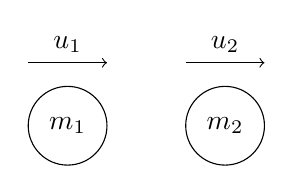
\begin{tikzpicture}
		\draw (-1,0) circle (0.5) node{$m_1$};
		\draw (1,0) circle (0.5) node{$m_2$};
		\draw[->] (-1.5,.8) -- (-0.5,.8) node[midway,above]{$u_1$};
		\draw[->] (0.5,.8) -- (1.5,.8) node[midway,above]{$u_2$};
		\end{tikzpicture}
		
		initial state before collision
	\end{center}
\end{minipage}
\begin{minipage}{0.5\textwidth}
	\begin{center}
		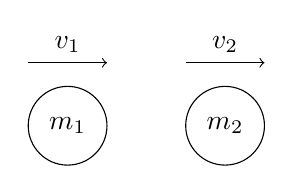
\begin{tikzpicture}
		\draw (-1,0) circle (0.5) node{$m_1$};
		\draw (1,0) circle (0.5) node{$m_2$};
		\draw[->] (-1.5,.8) -- (-0.5,.8) node[midway,above]{$v_1$};
		\draw[->] (0.5,.8) -- (1.5,.8) node[midway,above]{$v_2$};
		\end{tikzpicture}
		
		final state after collision
	\end{center}
\end{minipage}
\end{figure}

before and after collision, one has: $\boxed{m_1u_1 + m_2u_2 = m_1v_1 + m_2v_2}$

due to the vector nature of momentum, minus sign is needed if direction of motion reverses

\subsubsection{elastic \& inelastic collisions}

for inelastic collision, kinetic energy is lost to plastic deformation

for elastic collisions, no kinetic energy is lost: $\boxed{\frac{1}{2}m_1 u_1^2 + \frac{1}{2}m_2 u_2^2 = \frac{1}{2}m_1 v_1^2 + \frac{1}{2}m_2 v_2^2}$

together with momentum conservation, this reduces to $\boxed{u_1 - u_2 = v_2 - v_1}$

for elastic collision, relative speed of approach equals relative speed of separation 

for inelastic process, relative speed of separation is less than that of approach

\subsubsection{coefficient of restitution}

define coefficient of restitution as ratio of relative speeds before and after collision:
\begin{center}
$\boxed{e = \frac{v_2 - v_1}{u_1 - u_2}}$ or $\boxed{v_2 - v_1 = e(u_1 - u_2)}$
\end{center}

for elastic collision, $e = 1$; for inelastic collision, $0 < e < 1$

\vspace*{\baselineskip}

if an object collides at right angle with a fixed barrier with initial speed $u$

since barrier does not move, so $v-0 = e(0-u)$, then $v=-eu$

so object moves at speed $v=eu$ after collision, but with direction reversed



\example{Two small spheres $A$ and $B$ have masses $3m$ and $m$. They are projected towards each other with speeds $2u$ and $u$ relatively, the collision is perfectly elastic. What are their final speeds?}

momentum conservation: $3m\cdot 2u - m \cdot u = 3m v_A + m v_B$

relation for relative speeds: $v_B - v_A = 2u + u$

take simultaneous equations: $\Bigg\{\begin{array}{l}
3v_A + v_B = 5u \\
v_B - v_A = 3u
\end{array} \RA 
\Bigg\{\begin{array}{l}
v_A = \frac{1}{2}u \\
v_B = \frac{7}{2}u
\end{array}$

positive $v_A$ and $v_B$ means both spheres move in same direction as $u_A$ after collision \eoe

\example{Sphere $A$ of mass $m$ and sphere $B$ of mass $km$ are initially at rest. Sphere $A$ is projected towards $B$ with speed $u$, the restitution of collision is $\frac{1}{3}$. After the collision, sphere $A$ reverses. What is the possible range for value of $k$?}

{
	
\centering

$\Bigg\{\begin{array}{l}
mu + 0 = m v_A + km v_B \\
v_B - v_A = \frac{1}{3}(u-0)
\end{array} \RA
\Bigg\{\begin{array}{l}
	v_A + k v_B = u\\
	v_B - v_A = \frac{1}{3}u
\end{array} \RA 
\Bigg\{\begin{array}{l}
v_A = \frac{(3-k)u}{3(1+k)} \\
v_B = \frac{4u}{3(1+k)}
\end{array}$

}

sphere $A$ reverses so $v_A<0$ after collision $\RA \frac{(3-k)u}{3(1+k)}<0 \RA 3-k <0 \RA k>3$ \eoe

\example{Two small spheres $A$ and $B$ of masses $3m$ and $m$ lie on a smooth horizontal surface at rest. Sphere $A$ is projected towards $B$ with speed $u$. After the collision $B$ goes on to collide directly with a fixed smooth vertical barrier, before colliding with $A$ again. The coefficient of restitution between the spheres is $\frac{2}{3}$ and the coefficient of restitution between $B$ and the barrier is $e$. After the second collision between $A$ and $B$, the speed of $B$ is nine times the speed of $A$. Find the possible values of $e$.}

first collision between $A$ and $B$:

{
	
	\centering
	
	$\Bigg\{\begin{array}{l}
	3mu + 0 = 3m v_A + m v_B \\
	v_B - v_A = \frac{2}{3}(u-0)
	\end{array} \RA
	\Bigg\{\begin{array}{l}
	3v_A + v_B = 3u\\
	v_B - v_A = \frac{2}{3}u
	\end{array} \RA 
	\Bigg\{\begin{array}{l}
	v_A = \frac{7}{12}u \\
	v_B = \frac{5}{4}u
	\end{array}$
	
}

collsion between $B$ and the barrier: $v_B' = -ev_B \RA v_B' = -\frac{5e}{4}u$

second collision between $A$ and $B$:

{
	
	\centering
	
	$\Bigg\{\begin{array}{l}
	3mv_A + mv_B' = 3m w_A + m w_B \\
	w_B - w_A = \frac{2}{3}(v_A-v_B')
	\end{array} \RA
	\Bigg\{\begin{array}{l}
	3w_A + w_B = 3\cdot\frac{7}{12}u - \frac{5e}{4}u = \frac{7-5e}{4}u\\
	w_B - w_A = \frac{2}{3} \left(\frac{7}{12}u + \frac{5e}{4}u\right) = \frac{14+30e}{36}u
	\end{array}	$
	
	\vspace*{0.1\baselineskip}
	
	$4w_A = \frac{7-5e}{4}u-\frac{14+30e}{36}u = \frac{63-45e-14-30e}{36}u \RA w_A = \frac{49-75e}{144}u$
	
	\vspace*{0.1\baselineskip}
	
	$w_B = \frac{49-75e}{144}u + \frac{14+30e}{36}u = \frac{49-75e + 56 + 120e}{144}u \RA w_B = \frac{105+45e}{144}u $

}

given that $|w_B|=9|w_A|$, so $w_B = \pm 9 w_A$

{

\centering

$w_B = 9w_A \RA 105+45e = 9(49-75e) \RA e = \frac{9\times49-105}{9\times75+45}=\frac{336}{720} \RA e_1=\frac{7}{15}$

\vspace*{0.1\baselineskip}

$w_B = -9w_A \RA 105+45e = -9(49-75e) \RA e = \frac{9\times49+105}{9\times75-45}=\frac{546}{630} \RA e_2=\frac{13}{15}$

}

so two possible values of $e$ are $\frac{7}{15}$ and $\frac{13}{15}$ \eoe

\subsubsection{collision in two dimensions}

momentum should be conserved in any direction

so we can write down component equations

in particular, let's consider collision against a smooth barrier at angle $\theta$ to direction of motion

\begin{figure}[htp]
	\begin{center}
		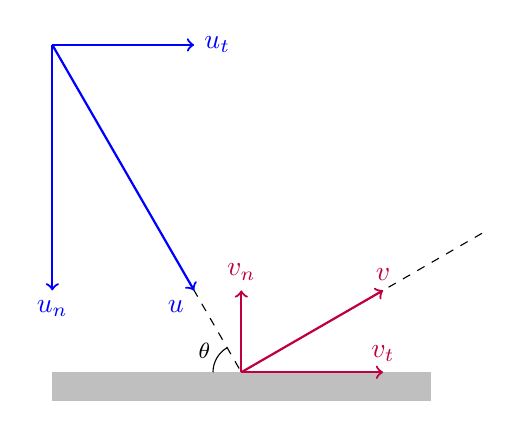
\begin{tikzpicture}[scale=1.2]
		\draw[gray!50,fill] (-2,-0.3) rectangle (2,0);
		\draw[dashed] (120:4) -- (0,0) -- (30:3);
		\draw[thick,blue,->] (120:4) --++ (-60:3) node[below left]{$u$};
		\draw[thick,purple,->] (0:0) --++ (30:1.732) node[above]{$v$};
		\draw[thick,blue,->] (120:4) --++ (1.5,0) node[right]{$u_t$};
		\draw[thick,blue,->] (120:4) --++ (0,-2.598) node[below]{$u_n$};
		\draw[thick,purple,->] (0:0) --++ (0:1.5) node[above]{$v_t$};
		\draw[thick,purple,->] (0:0) --++ (90:0.866) node[above]{$v_n$};
		\draw (120:0.3) arc(120:180:0.3);
		\node at (150:0.45) {{\footnotesize $\theta$}};
		\end{tikzpicture}
	\end{center}
\end{figure}

there is contact force normal to barrier, so there is change of momentum in this direction

change in normal component of velocity depends on coefficient of restitution

barrier is smooth, i.e., no tangential force, so no change in tangential momentum

tangential component of velocity remains unchanged after collision

components of velocity before and after collisions are: 

{

\centering

$v_t = u_t = u\cos\theta$, $\quad v_n = eu_n = eu \sin\theta$

}



\example{A sphere hits a smooth vertical barrier at $60^\circ$ to the direction of motion. In the impact with the wall, the sphere loses $\frac{2}{3}$ of its kinetic energy. Find the coefficient of
restitution between the sphere and the wall.}

components of velocity before collision are: 

{

\centering

$u_t = u\cos60^\circ = \frac{1}{2}u, \quad u_n = u\sin60^\circ = \frac{\sqrt{3}}{2}u$

}

components of velocity after collision are: 

{

\centering

$v_t = u_t = \frac{1}{2}u, \quad v_n = eu_n = \frac{\sqrt{3}}{2}eu$

$v^2 = v_t^2 + v_n^2 = \frac{1}{4}u^2 + \frac{3}{4}e^2u^2 = \frac{1+3e^2}{4}u^2$

}

$\frac{2}{3}$ of K.E. is lost, so $\frac{1}{2}mv^2 = \frac{1}{3} \cdot \frac{1}{2}mu^2$, or $v^2 = \frac{1}{3} u^2$, therefore

{
	
\centering
	
$\frac{1+3e^2}{4}u^2 = \frac{1}{3}u^2 \RA 1+3e^2 = \frac{4}{3} \RA e=\frac{1}{3}$ 
	
}
